%%%%%%%%%%%%%%%%%%%%%%%%%%%%%%%%%%%%%%%%%%%%%%%%%%%%%%%%%%%%%%%%%%%%%%%%%%
%                                                                        %
%                            INTRODUCTION                                %
%                                                                        %
%%%%%%%%%%%%%%%%%%%%%%%%%%%%%%%%%%%%%%%%%%%%%%%%%%%%%%%%%%%%%%%%%%%%%%%%%%
\subsection*{}
\begin{frame}{Ability to Detect Signal}
  \textbf{How is the light collected from the detector}
  \vspace{1cm}
  \begin{itemize}
    \item Not all of the detectors are optically transparent
    \item Light collection strategies:
    \begin{itemize}
      \item Pipe the light out along the edge?
      \item Use wavelength shifters?
      \item How much spacing is needed between layers?
    \end{itemize}
    \item Is it possible to design a workable detector?
  \end{itemize}
\end{frame}
%%%%%%%%%%%%%%%%%%%%%%%%%%%%%%%%%%%%%%%%%%%%%%%%%%%%%%%%%%%%%%%%%%%%%%%%%%
\begin{frame}[fragile]{Large Area Scintillators}
\begin{itemize}
  \item Simulations have been completed for a large area transparent scintillator
  \item Two orders of magnitude drop in the number of photons \SI{90}{\cm} from the distance of emission\cite{riggi_introducing_2011}
  \item Parameter studies on different types of light guides
\end{itemize}
\begin{table}
  \centering
  \caption[PNNL Light Collection Efficiencies]{Light collection efficiencies of several detector designs simulated by PNNL\cite{pnnl_14283}.}
  \label{tab:PNNLLightCollectionEfficiency}
  \begin{tabular}{c|c c}
  \toprule
  & \multicolumn{2}{c}{Light Collection Efficiency} \\
  Number of PMTs  & 2-in PMT & 5-in PMT \\
  \midrule
  2 & 7.0\% & 18.8\% \\
  4 & 13.3\% & 30.7\ \\
  6 & 18.4\% & 40.2\% \\
  \bottomrule
  \end{tabular}
\end{table}
\end{frame}
%%%%%%%%%%%%%%%%%%%%%%%%%%%%%%%%%%%%%%%%%%%%%%%%%%%%%%%%%%%%%%%%%%%%%%%%%%
%%%%%%%%%%%%%%%%%%%%%%%%%%%%%%%%%%%%%%%%%%%%%%%%%%%%%%%%%%%%%%%%%%%%%%%%%%
%                                                                        %
%                             PROPOSED WORK                              %
%                                                                        %
%%%%%%%%%%%%%%%%%%%%%%%%%%%%%%%%%%%%%%%%%%%%%%%%%%%%%%%%%%%%%%%%%%%%%%%%%%
\subsection{Proposed Work}
\begin{frame}{Proposed Work}
  \textbf{Neutronics, energy deposition, and light transport}
  \vspace{0.5cm}
  \begin{columns}[onlytextwidth]
    \begin{column}{0.45\textwidth}
      Geometries
      \begin{itemize}
        \item GS2O  (with and without reflector)
        \item 4 in by 6 in two layer detectors
        \item Full RPM
      \end{itemize}
    \end{column}
    \begin{column}{0.45\textwidth}
      Parameter Studies
      \begin{itemize}
        \item Light guide thickness
        \item Light guide material (WLS)
        \item Reflectivity and wrappings
      \end{itemize}
    \end{column}
  \end{columns}
  \vspace{0.5cm}
  \textbf{Optimization Techniques}
  \vspace{0.5cm}
  \begin{itemize}
    \item Multi-variate optimization for parameter study
    \item Genetic Algo for layering
  \end{itemize}
\end{frame}
%%%%%%%%%%%%%%%%%%%%%%%%%%%%%%%%%%%%%%%%%%%%%%%%%%%%%%%%%%%%%%%%%%%%%%%%%%
%                                                                        %
%                               METHODS                                  %
%                                                                        %
%%%%%%%%%%%%%%%%%%%%%%%%%%%%%%%%%%%%%%%%%%%%%%%%%%%%%%%%%%%%%%%%%%%%%%%%%%
\subsection{Methods}
\begin{frame}[fragile]{Light Transport in GEANT4}
\begin{itemize}
  \item GEANT4 examples: \verb+ExampleN06+,\verb+extended/LXe+, \verb+extended/WLS+
  \item Sensitive detector on PMT
  \item Timing information
  \item Material Properties
  \small
  \begin{itemize}
    \item Optical absorption
    \item Index of refraction
    \item Surface properties - optical surface model \cite{5485130}
  \end{itemize}
\end{itemize}
\end{frame}
\begin{frame}[fragile]{Optical Material Properties}
Most difficult part of simulation is correct properties
\begin{lstlisting}
void Materials::SetOpticalPropertiesGS20(){
    // Index of Reflection (146 nm to 1570 nm)
    const G4int nRINDEX = 13;
    G4double photonEnergyRINDEX[nRINDEX] = 
    {8.550*eV,4.723*eV,3.262*eV,2.492*eV,2.016*eV,
    1.692*eV,1.458*eV,1.281*eV,1.142*eV,1.031*eV, 
    0.939*eV,0.862*eV,0.797*eV};
    G4double RefractiveIndexGlass[nRINDEX]=
    {1.6508,1.5266,1.4980,1.4872,1.4819,    
    1.4790,1.4772,1.4760,1.4752,1.4746,    
    1.4742,1.4738,1.4736};
    // Absorbition Length
    const G4int nABS=2;
    G4double photonEnergyABS[nABS] = {3.5*eV,1.75*eV};
    G4double AbsLengthGlass[nABS] = {70*cm, 70*cm};  
\end{lstlisting}
\end{frame}
\begin{frame}[fragile]{Optical Material Properties}
\begin{lstlisting}
    G4double photonEnergyEM[nEM] = {3.8,3.5,3.1,2.8,2.5};
    G4double emGS20[nEM]={0,0.19,0.37,0.32,0.10,0.02};
    MPTGS20->AddProperty("RINDEX",photonEnergyRINDEX,RefractiveIndexGlass,nRINDEX);
    MPTGS20->AddProperty("ABSLENGTH",photonEnergyABS,AbsLengthGlass,nABS);
	  MPTGS20->AddProperty("FASTCOMPONENT",photonEnergyEM,emGS20,nEM);
    MPTGS20->AddConstProperty("FASTTIMECONSTANT",50*ns);
    MPTGS20->AddConstProperty("SCINTILLATIONYIELD", 3600*MeV);
    MPTGS20->AddConstProperty("YIELDRATIO", 1.0);
    MPTGS20->AddConstProperty("RESOLUTIONSCALE", 1.0);
}
\end{lstlisting}
\end{frame}
%%%%%%%%%%%%%%%%%%%%%%%%%%%%%%%%%%%%%%%%%%%%%%%%%%%%%%%%%%%%%%%%%%%%%%%%%%
%                                                                        %
%                          PRELIMARY RESULTS                             %
%                                                                        %
%%%%%%%%%%%%%%%%%%%%%%%%%%%%%%%%%%%%%%%%%%%%%%%%%%%%%%%%%%%%%%%%%%%%%%%%%%
\subsection{Preliminary Results}
\begin{frame}{Small Scale Detectors}
\begin{table}
  \centering
  \caption[Simulated and Measured Light Yields]{Simulated and Measured Light Yields}
  \begin{tabular}{m{2cm}| m{2cm} m{2cm} m{2cm}}
  \toprule
  & EJ-426 & PS Film A & PS Film B \\
  \midrule
  Simulated & 2,100 & 180 & 130 \\
  Measured & 1,500 & 220 & 100 \\
  Relative Error & 40\% & -18\% & 30\% \\
  \bottomrule
  \end{tabular}
\end{table}
\begin{itemize}
  \item Current work on ensuring correct selection of parameters
\end{itemize}
\end{frame}
%%%%%%%%%%%%%%%%%%%%%%%%%%%%%%%%%%%%%%%%%%%%%%%%%%%%%%%%%%%%%%%%%%%%%%%%%%
\begin{frame}{Simulated GS20}
  \begin{columns}[onlytextwidth]
    \begin{column}{0.55\textwidth}
      \begin{itemize}
        \item Collection efficiency with teflon: 92\%
        \item Collection efficiency with black tape: 64\%
        \item Simulation and measurements agree
      \end{itemize}
    \end{column}
    \begin{column}{0.4\textwidth}
      \begin{figure}
        \vspace*{-1cm}
        \begin{subfigure}[b]{\textwidth}
        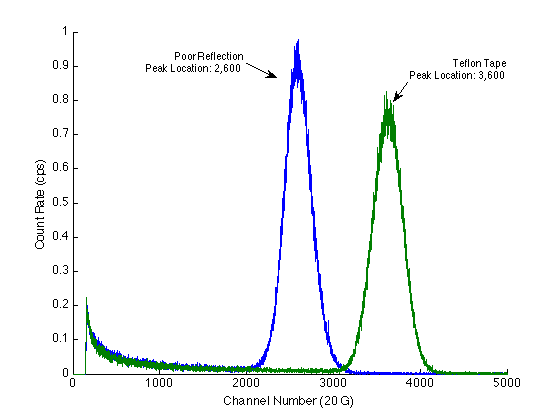
\includegraphics[width=\textwidth]{GS20_TeflonBlackTape.png}
        \end{subfigure}
        
        \begin{subfigure}[b]{\textwidth}
        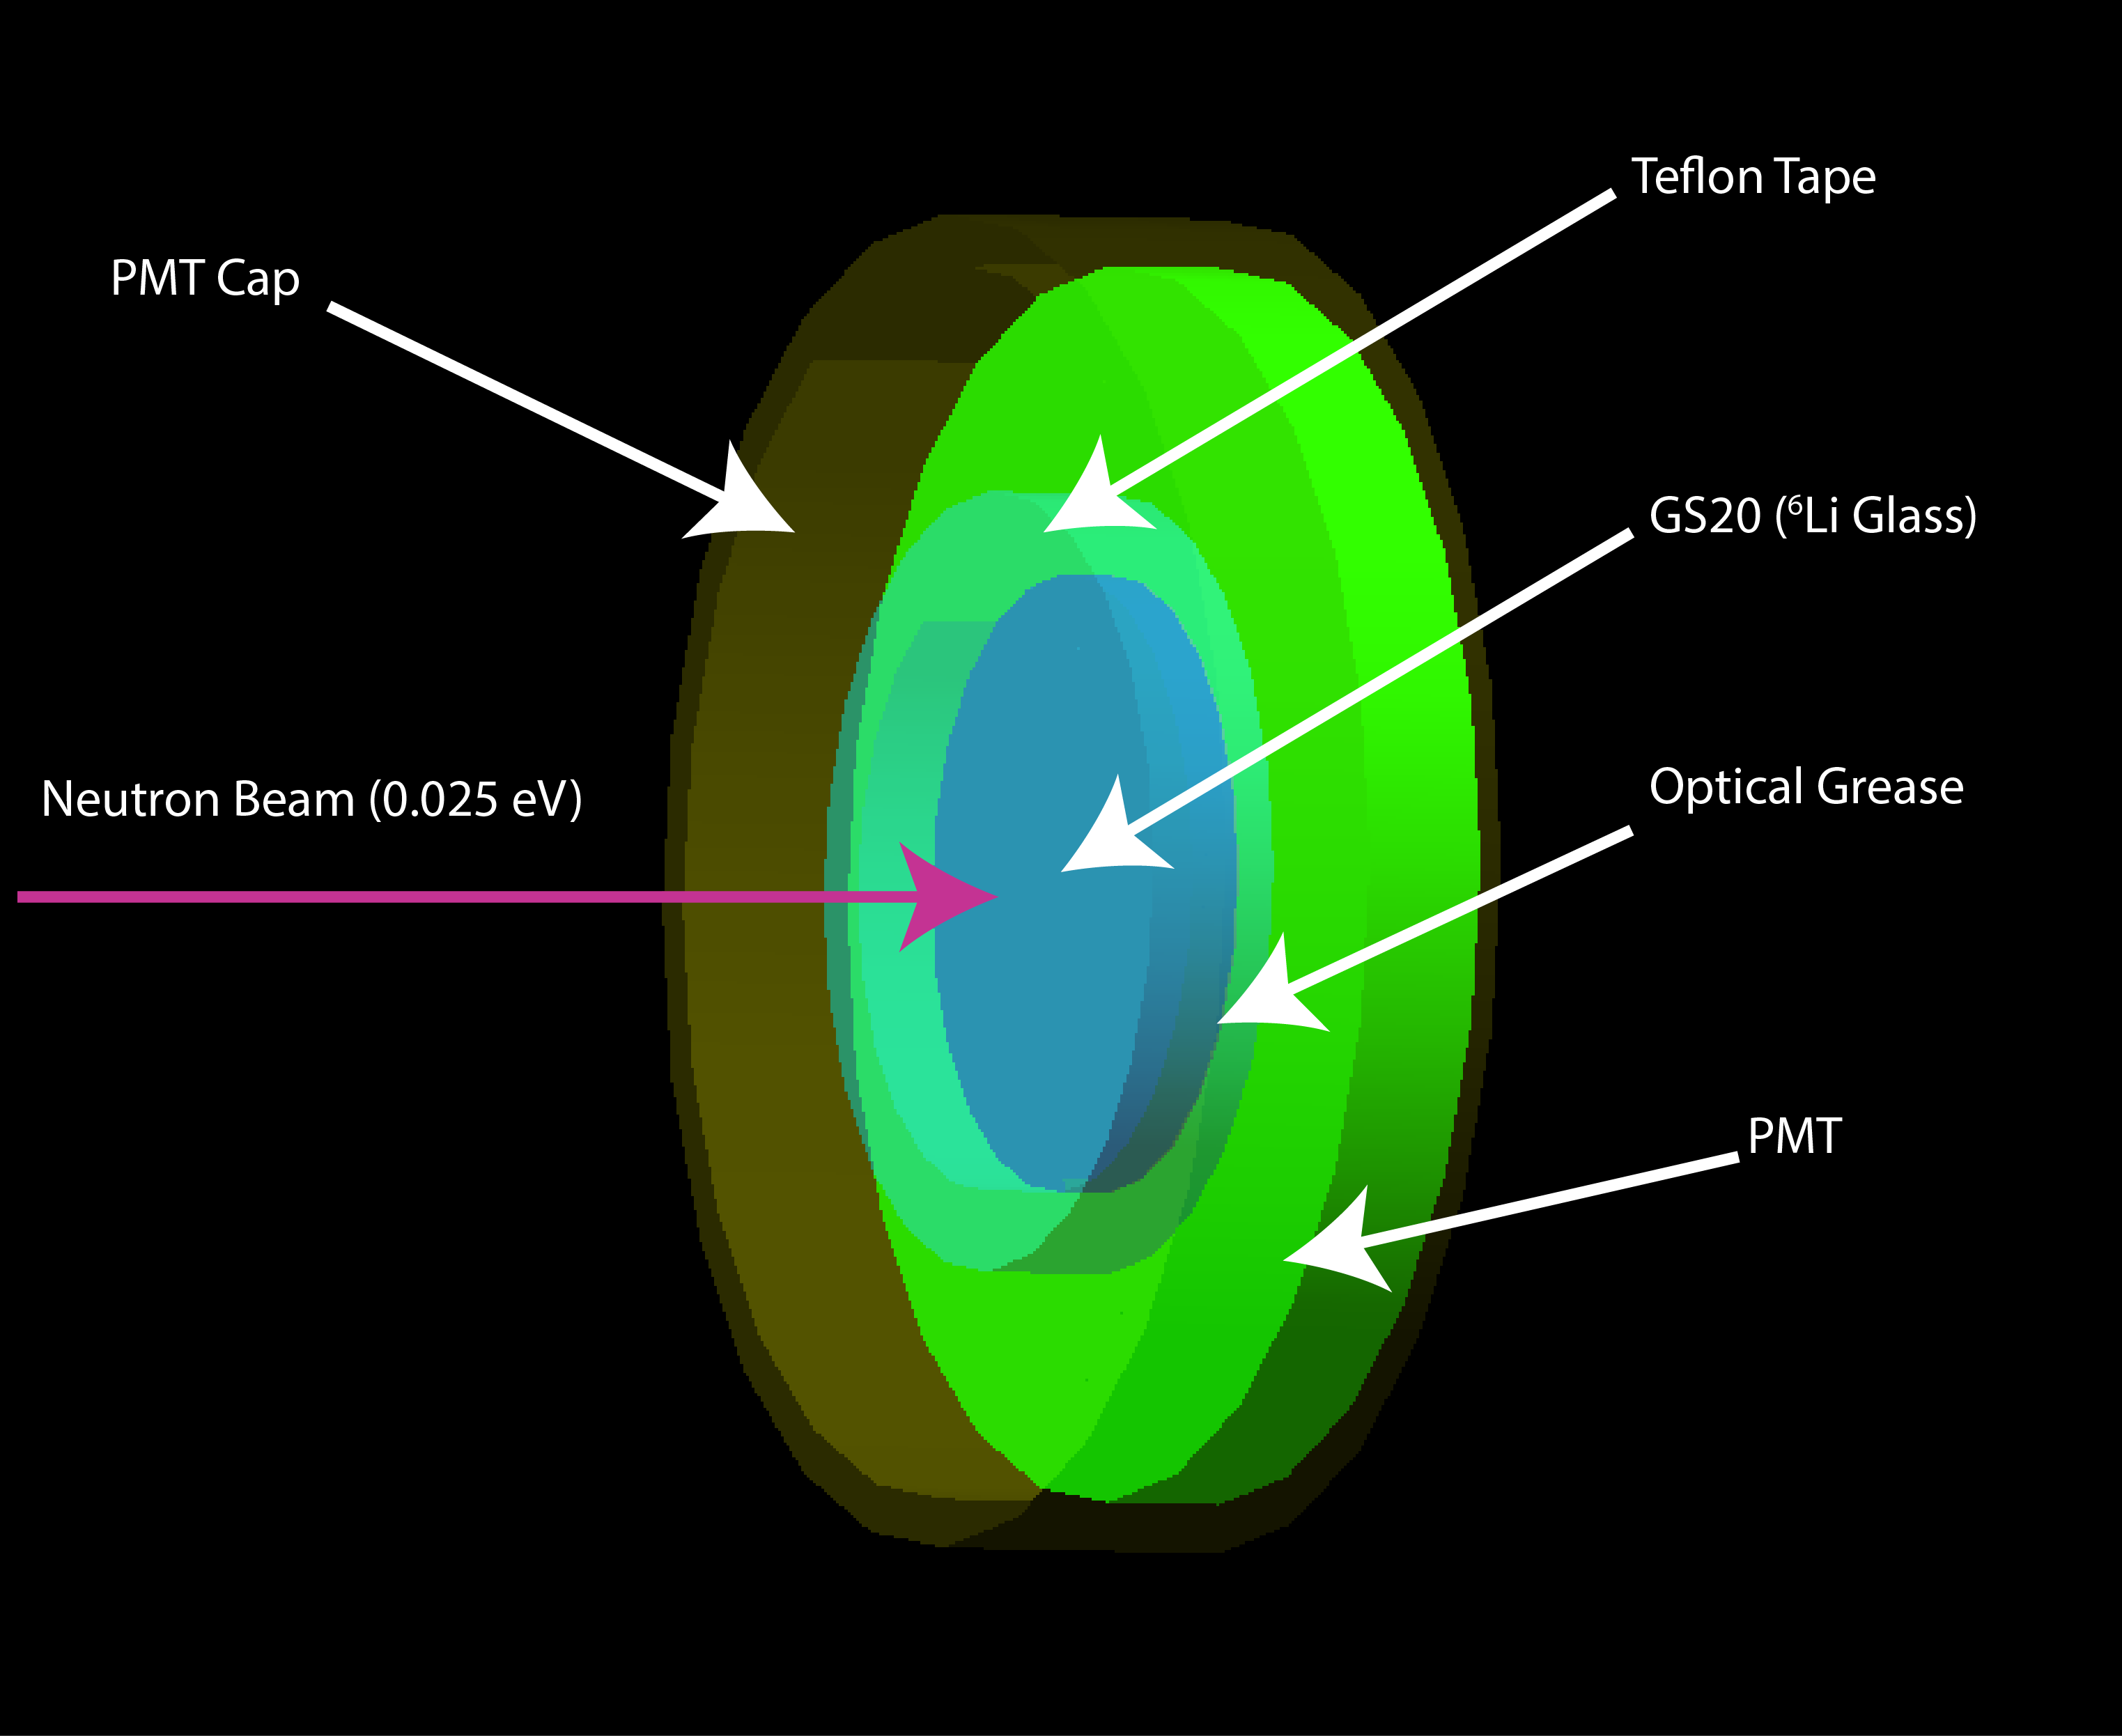
\includegraphics[width=\textwidth]{GEANT4AnnotatedGeo_GS20SimGeo.png}
        \end{subfigure}
      \end{figure}
    \end{column}
  \end{columns}
\end{frame}
%%%%%%%%%%%%%%%%%%%%%%%%%%%%%%%%%%%%%%%%%%%%%%%%%%%%%%%%%%%%%%%%%%%%%%%%%%
\begin{frame}{Simulated RPM}
  \begin{columns}[onlytextwidth]
    \begin{column}{0.45\textwidth}
		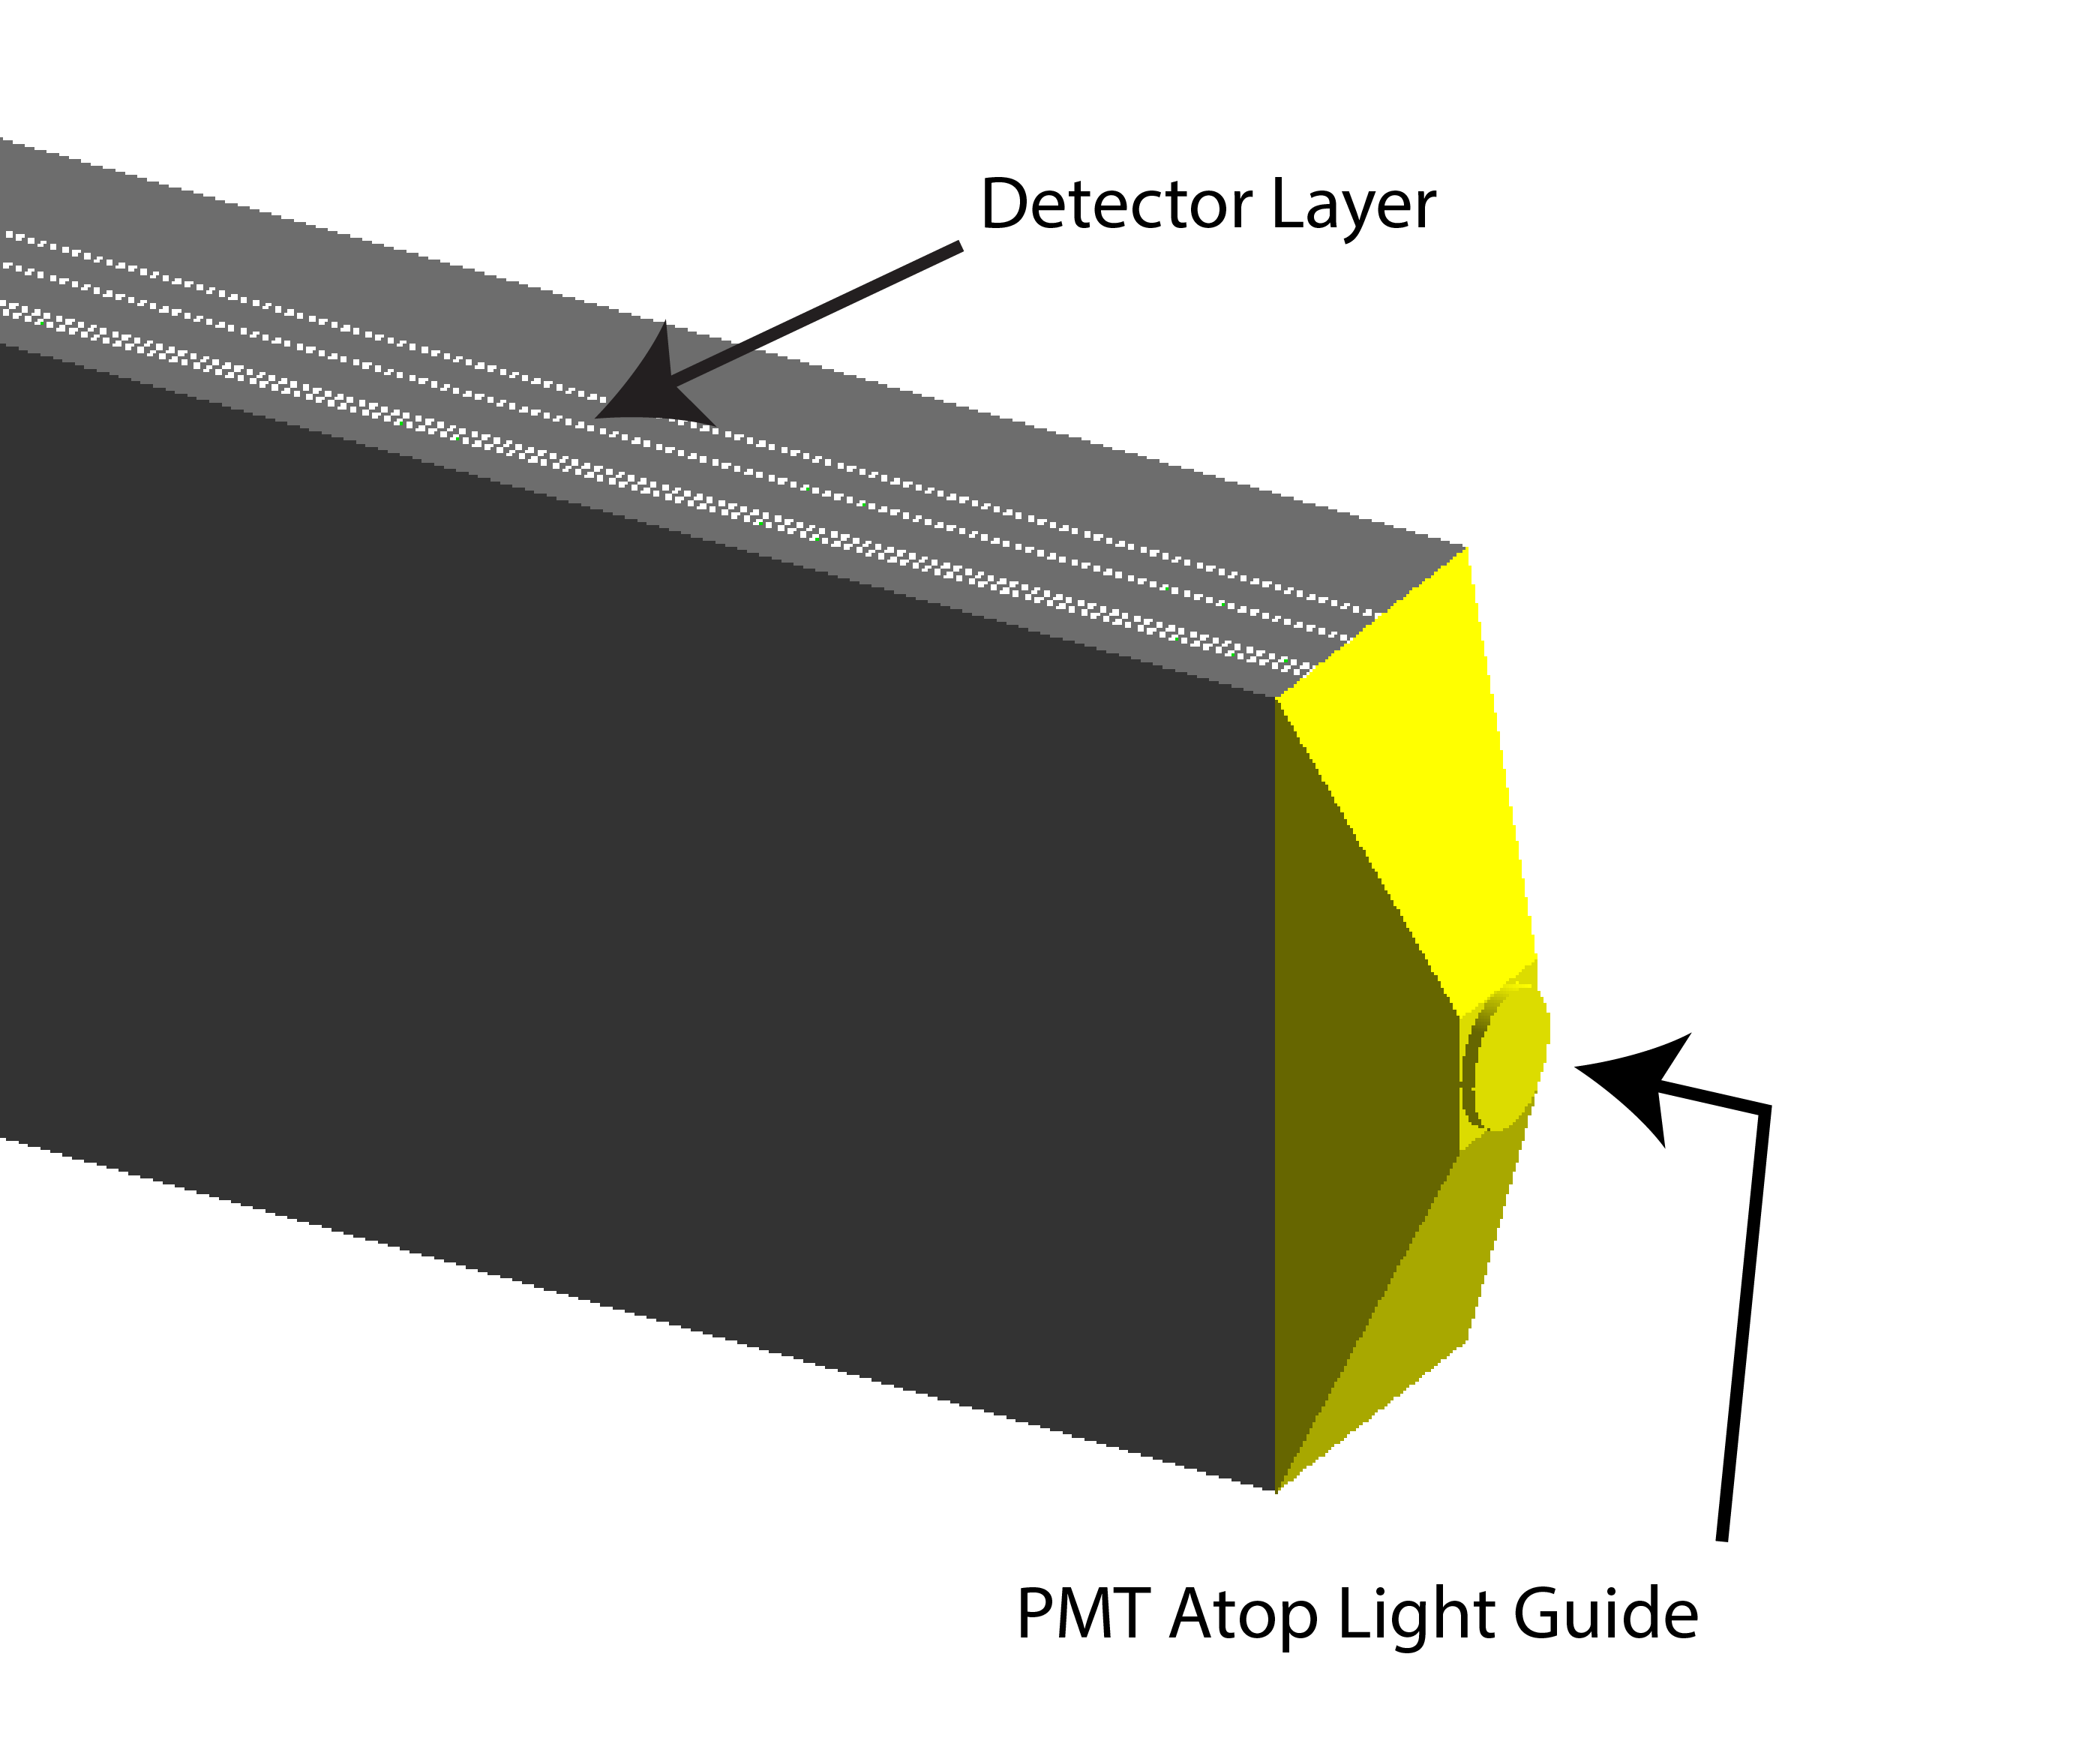
\includegraphics[width=\textwidth]{GEANT4AnnotatedGeo_RPM8SimGeoPMTEnd.png}
    \end{column}
    \begin{column}{0.45\textwidth}
		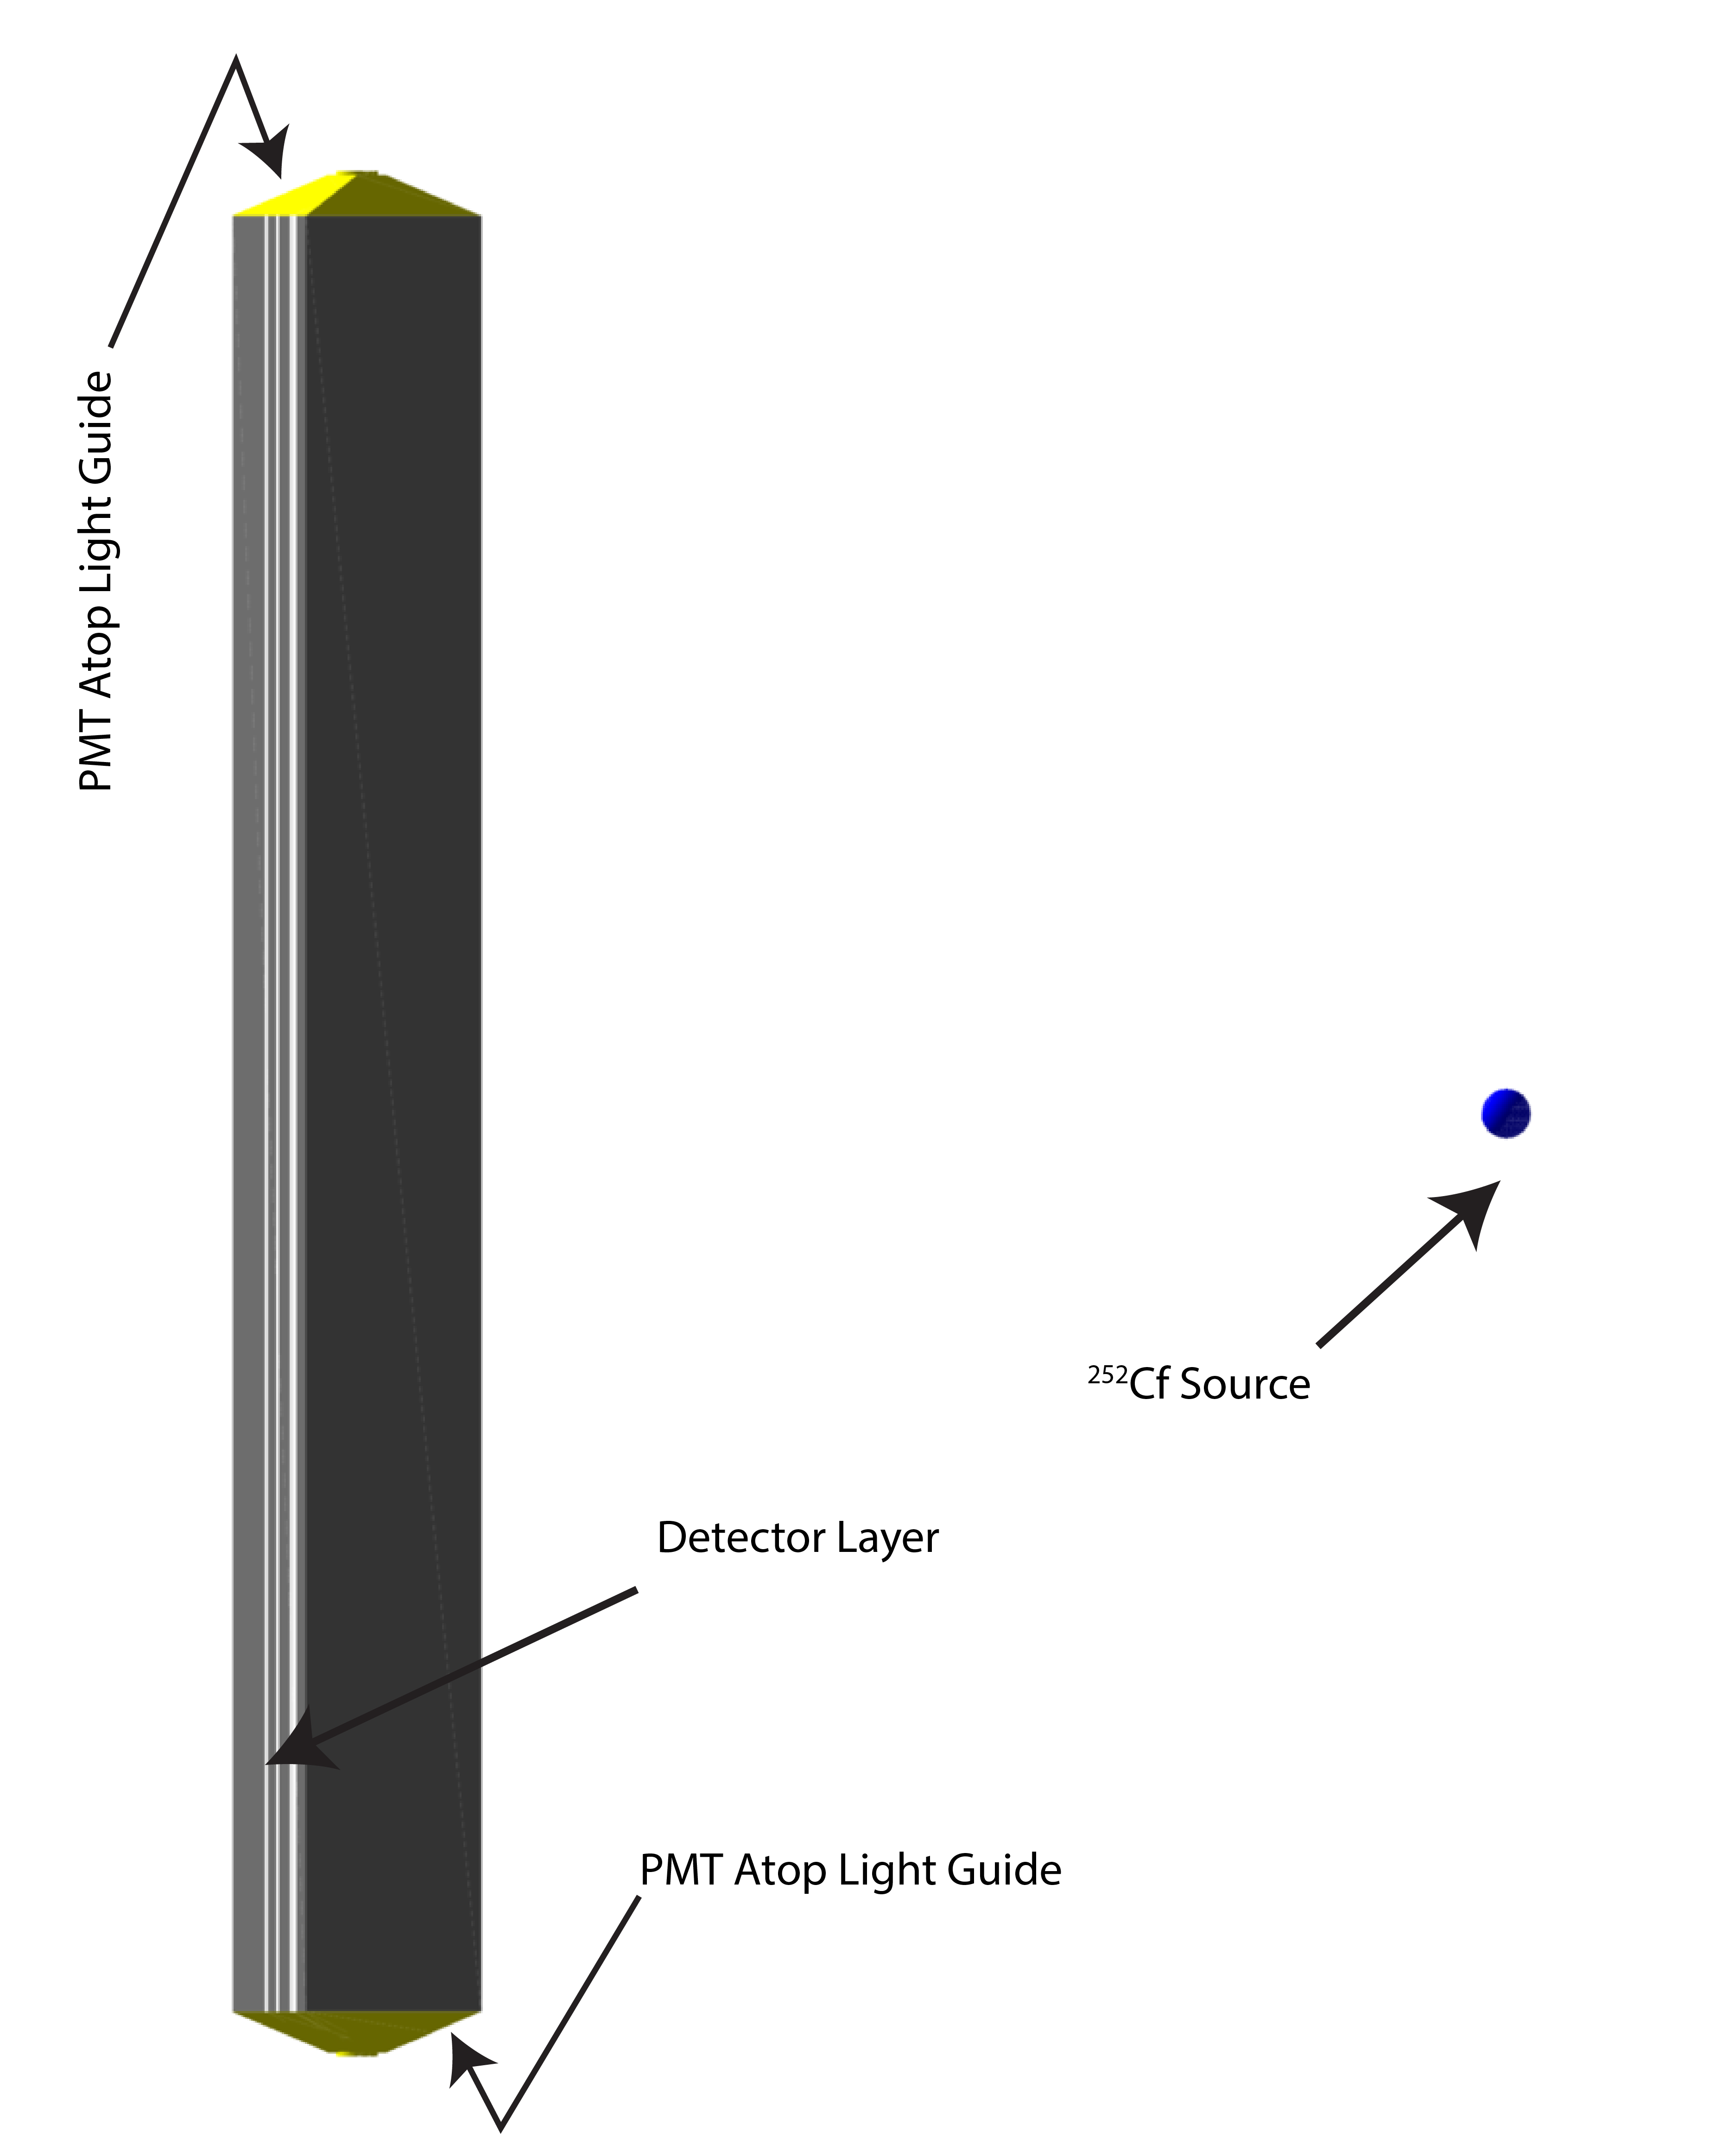
\includegraphics[width=\textwidth]{GEANT4AnnotatedGeo_RPM8SimGeo.png}
    \end{column}
  \end{columns}
\end{frame}
%%%%%%%%%%%%%%%%%%%%%%%%%%%%%%%%%%%%%%%%%%%%%%%%%%%%%%%%%%%%%%%%%%%%%%%%%%
